%chapter 6
\chapter{Freight Transport Operation}
%
Some important terminologies:
\begin{enumerate}
	\item \textbf{\textit{Transport}} is the actual movement of goods from one location to another using a means or a vehicle of transport (e.g. trains, trucks, boats) and a transport infrastructure (e.g. roads, railways, canals).
	\item \textbf{\textit{Distribution}} often denotes all activities relevant to physical movement of goods, including transportation, but also transhipment and warehousing.
	\item \textbf{\textit{Logistics}} is generally used as an overarching term that includes all activities related to the movement and coordination of goods from their source of origin to the final point of delivery, and includes production and distribution. Here, movement does not just correspond to physical movement of goods but also the flow of information.
\end{enumerate}
%
\section{Main Actors of Freight Transport and Distribution}
While freight transport and distribution include many elements, including various organizations and people, the three fundamental actors who actively take part in the domain are described here.
\subsection{Shippers}
The demand for freight transportation is generated by shippers. Each shipper will have their own logistics strategy, which includes whether to operate their own fleet or to use an external party to which it will outsource their logistics and distribution activities, as well as choosing the mode(s) of transport. The process through which the shippers will define their logistics activities generally takes a three-level decision structure:
\begin{enumerate}
	\item The long-term decisions in the first level involve defining strategies in line with their customer network and production activities.
	\item The second-level medium-term decisions include levels of inventories at production, warehousing, and distribution facilities, frequency and amount of shipping and flexibility of service.
	\item At the short-term level, shippers decide on the attributes of the services required for its shipments, such as maximum rates, transport time, reliability and safety.
\end{enumerate}
%
In making these decisions, they will consider the availability and the characteristics of the services offered on the market by carriers and intermediaries, such as freight brokers and third-party logistics providers.
%%
\subsection{Carriers}
Carriers are people, businesses or organisations that operate and offer transportation services for shippers. They may either provide a customised service, where a vehicle or a fleet will be dedicated exclusively to a particular customer, or operate on the basis of consolidation, where each vehicle contains several pieces of freight for different customers with possibly different origins and destinations. In the latter case, carriers generally operate their services according to a published timetable, which prescribes routes, schedules and rates they offer.
%%
\subsection{Intermediaries}
In some cases, the shipper operates their own fleets of vehicles and does not require an external carrier to ship goods on their behalf. In this case, the management of the relevant transportation and distribution is done inhouse. If a shipper does not own a fleet, then it may choose to work directly with one or several carriers.
\paragraph{}
Shippers may alternatively use a freight forwarder, an intermediary person or organization that acts as a third party and manages the shipments on behalf of the shipper by contracting one or several carriers. They also help to identify a suitable mode or a combination of modes for the shipper. Freight forwarders work closely with shippers and carriers, as well as other entities in the transportation network, such as ports or terminals, particularly if they additionally undertake ancillary services such as customs clearance.
%%
\section{Modes of Transportation}
There exist different means of transporting freight over the network, each of which is referred to as a mode of transport. Transportation modes can be differentiated with respect to the type and specification of the vehicle used, the underlying technology, the relevant infrastructure and the nature of the associated operations. The three main modes of transport are air (e.g., cargo planes), land (including road, rail and off-road) and water (e.g., ships in oceans, barges in rivers). Other modes of transport, such as pipelines (e.g., to transport gas) and cable transport (e.g., elevators and cable-cars), also exist.
\paragraph{}
The term mode can also be used to denote different types of vehicles
within a given domain of transport. For example, trucks, vans and bicycles can be seen as three separate modes operating within road transportation due to their distinct features, such as different capacities, capabilities and restrictions. In this example, trucks have the largest capacity but often have restrictions in traveling in urban areas, whereas bicycles are much smaller in capacity but do not suffer from the same type of restrictions as trucks or vans. Brief descriptions of the three main modes of transportation are explained here.
%
\subsection{Road}
Road has been, and continues to be, the most widely used mode of freight transport, both nationally and globally. One of the main reasons behind its popularity is the ability of road transport to offer a very quick service and often be available on demand.
\paragraph{}
A wide variety of vehicles are used for road freight transportation, which
can be differentiated on the basis of size, capacity, weight and the type of energy used. Vehicle classification on road transportation is generally based on the Gross Vehicle Weight Rating (GVWR), which refers to the maximum allowable total weight of a vehicle including its empty mass, fuel and any load carried. The empty mass of the vehicle, but with fuel and fluids such as engine oil, is named as the curb weight. Vehicle classifications vary from one country to another. In the United States, eight classes exist, with vehicles in the lightest class having a GVWR up to around 3 tonnes, and those in the heaviest class with a GVWR higher than 15 tonnes. In the United Kingdom, more classes exist, with those of at most 3.5 tonnes gross weight described as light goods vehicles (LGVs) and those between 3.5 and 44 tonnes gross weight named as lorries or heavy goods vehicles (HGVs).
\paragraph{}
Most vehicles used in road freight transportation run on gasoline or diesel engines. Vehicles using alternative sources of fuel or energy have also been developed, such as those running on batteries, biofuels (such as bioalcohol or ethanol), biodiesel, compressed natural gas, hydrogen, and liquefied petroleum gas (LPG), for use in freight distribution. Within urban areas, human-powered vehicles, such as bicycles and tricycles, can also be used for goods deliveries. To overcome the sole dependency on human power, some of the freight bicycles have power assist motors to aid the cyclist.
\paragraph{}
The road network is composed of motorways (or highways), urban roads,
rural roads, lanes or graded roads and includes bridges and tunnels. Traffic on the road network is controlled by means of traffic signals, signs or markings on the pavement. Various legal requirements are imposed on freight vehicles traveling on the road network, which include limitations on vehicle weight, dimensions, mandatory equipment, licenses and insurances. As for truck drivers, there also exist regulations on driving and working hours, which restrict the duration of driving time and require break and rest periods in long-haul journeys. These regulations aim at reducing driver fatigue, which is known to have adverse affects on road and driver safety. The regulations usually differentiate between on-duty time, which is the time spent working, including driving, waiting, loading and unloading and doing paperwork, and off-duty time, where the driver has no obligation to work. In the United States, for example, these regulations are known as Hours of Service, which limit the maximum consecutive driving time between two rest periods to 11 hours, at which point the driver must be off-duty for at least 10 consecutive hours. Furthermore, a truck driver cannot drive if 8 hours or more have elapsed since the end of the last off-duty period of at least 30 minutes. Similar regulations prevail in other countries, albeit with differences.
%
\subsection{Rail}
Rail freight transportation is known for its ability to offer cost-effective long-haul transportation services, primarily, but not exclusively, for bulk cargo. There are two major components of a rail system, namely the rail network infrastructure and freight trains.
\paragraph{}
The rail network is a large and complex structure composed of nodes and
tracks (or track segments) as links between the nodes. The former include yards or terminals where classification or marshalling operations are performed, stations where cargo is picked up from or delivered to and junctions that are signal-controlled points in the rail network to allow trains to switch from one route to another.
\paragraph{}
Freight trains are composed of one or more locomotives, and several rail
wagons (or cars). Locomotives move the train along the tracks by either pulling it from the front or push from the rear and range from the earlier types powered by steam to contemporary ones using electricity, magnetic force or diesel engine. Rail wagons carry the freight and come in a variety of forms, including specialized wagons for carrying particular types of cargo (e.g., autoracks for carrying automobiles or refrigerator cars for temperature-sensitive goods). A train is characterized by its route, origin, destination, intermediate stops, the physical path it travels on and the schedule information that includes departure and arrival times at each station where it stops. Each wagon also has an itinerary that specifies an origin and a destination station and need not correspond to the origin and destination of the train on which it is carried. Wagons may travel on several trains during their journey, usually in groups called blocks. Each block is assigned an origin and a destination, although individual cars in a single block may have different origins and destinations. A block is treated as a single unit for handling purposes. Once formed at its origin yard, a block will not be classified again until it arrives at its destination yard.
\paragraph{}
Classification or marshalling refers to a set of operations carried out at
yards or terminals, where incoming trains are disassembled by decoupling the rail cars and new trains are formed using individual cars or blocks. Bekta¸s et al. (2009) provide a detailed description of the operations at a classification yard, according to which a train arriving at a yard first enters a receiving area, where the engines are taken away for inspection and maintenance, blocks are separated and cars are inspected. The classification operation begins from this point on and can be performed in two ways, depending on the type of the rail yard. In flat yards, a switching engine is used to push a group of cars out of the receiving tracks onto one of the classification tracks. In hump yards, classification is performed by using an artificially built hill, called the hump, where an engine pushes a group of cars out of the receiving area and up the ramp until it reaches the top of the hill. Due to the pull of the gravitational force, the cars roll down the incline on the other side of the hump, usually one car at a time, and are directed onto one of the classification tracks. Following this operation, each classification track becomes occupied by a group of cars that form the block. Each block then waits until the departure time of its outbound train. When the train is due to leave, they are pulled out of the classification tracks onto the departure tracks and are attached to the train. Following one last inspection of the whole train, the train and blocks leave the yard. The figure below shows the general structure of a classification hump yard.
%
\begin{center}
	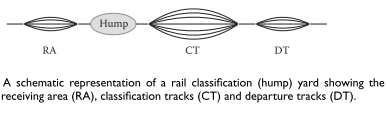
\includegraphics[scale=0.7]{gfx/fig33.png}
\end{center}
\paragraph{}
Classification is not the only operation that is performed at a rail yard.
Other types of operations include inspection, crew change, refueling the trains and dropping and picking up blocks of cars. Among these, however, classification is known to be the major time-consuming operation.